%% LyX 2.0.8.1 created this file.  For more info, see http://www.lyx.org/.
%% Do not edit unless you really know what you are doing.
\documentclass[12pt,english,british]{scrartcl}
\usepackage[T1]{fontenc}
\usepackage[latin9]{inputenc}
\usepackage{amsthm}
\usepackage{amsmath}
\usepackage{amssymb}
\usepackage{graphicx}
\usepackage[numbers]{natbib}

\makeatletter
%%%%%%%%%%%%%%%%%%%%%%%%%%%%%% Textclass specific LaTeX commands.
\theoremstyle{plain}
\newtheorem{thm}{\protect\theoremname}[section]
  \theoremstyle{definition}
  \newtheorem{defn}[thm]{\protect\definitionname}
  \theoremstyle{plain}
  \newtheorem{lem}[thm]{\protect\lemmaname}
  \theoremstyle{plain}
  \newtheorem{cor}[thm]{\protect\corollaryname}
  \theoremstyle{plain}
  \newtheorem{prop}[thm]{\protect\propositionname}

%%%%%%%%%%%%%%%%%%%%%%%%%%%%%% User specified LaTeX commands.
\usepackage{icml2016} 

%\usepackage[accepted]{icml2016}

\makeatother

\usepackage{babel}
  \addto\captionsbritish{\renewcommand{\corollaryname}{Corollary}}
  \addto\captionsbritish{\renewcommand{\definitionname}{Definition}}
  \addto\captionsbritish{\renewcommand{\lemmaname}{Lemma}}
  \addto\captionsbritish{\renewcommand{\propositionname}{Proposition}}
  \addto\captionsbritish{\renewcommand{\theoremname}{Theorem}}
  \addto\captionsenglish{\renewcommand{\corollaryname}{Corollary}}
  \addto\captionsenglish{\renewcommand{\definitionname}{Definition}}
  \addto\captionsenglish{\renewcommand{\lemmaname}{Lemma}}
  \addto\captionsenglish{\renewcommand{\propositionname}{Proposition}}
  \addto\captionsenglish{\renewcommand{\theoremname}{Theorem}}
  \providecommand{\corollaryname}{Corollary}
  \providecommand{\definitionname}{Definition}
  \providecommand{\lemmaname}{Lemma}
  \providecommand{\propositionname}{Proposition}
\providecommand{\theoremname}{Theorem}

\begin{document}
\twocolumn[ \icmltitle{Fancy title}
% It is OKAY to include author information, even for blind
% submissions: the style file will automatically remove it for you
% unless you've provided the [accepted] option to the icml2015
% package.
\icmlauthor{Kacper Chwialkowski$^*$}{kacper.chwialkowski@gmail.com}
\icmlauthor{Heiko Strathmann$^*$}{heiko.strathmann@gmail.com}
\icmlauthor{Arthur Gretton}{arthur.gretton@gmail.com}
\icmladdress{Gatsby Unit, University College London, United Kingdom}
% You may provide any keywords that you 
% find helpful for describing your paper; these are used to populate
% the "keywords" metadata in the PDF but will not be shown in the document
\icmlkeywords{kernels, statistical testing}
\vskip 0.3in ]

\begin{abstract}
We present a kernel one-sample test. Given a set of samples, the test
allows to quantify how likely it is that the samples have been generated
from a given probability density function. Our work extends recent
work on using Stein operators to construct goodness-of-fit metrics
\citep{gorham2015measuring}. Via phrasing the problem in the framework
of Reproducing Kernel Hilbert Spaces, we do not only achieve largely
improved computational properties, but also avoid the need for extra
knowledge of the density -- our metric solely depends on gradients
of the log-density. We analyse asymptotic properties of the metric
and embed it into the statistical hypothesis testing framework --
including efficient test constructions. As a demonstration of the
test's practicality, we apply it to quantifying convergence of approximate
Markov Chain Monte Carlo methods, statistical model critisism, and
checking estimation and approximation convergence in non-parametric
density estimation.
\end{abstract}
\selectlanguage{english}%
\global\long\def\ev{\mathbb{E}}


\selectlanguage{british}%

\section{Introduction}

Blablabla

\selectlanguage{english}%
The purpose of a goodness of fit test is to show whether a distribution
$p$ matches some reference distribution $q$, which is in our case
assumed to have a density wrt the Lebesgue measure, $dq(x)=q(x)dx$
(in fact, as we will see, it makes most sense for it to be in the
exponential family).


\section{Kernel One Sample Test}

In the following section we derive kernel one sample test. The test
is applicable to family distributions on Euclidean space $\mathcal{P}$,
where $p\in\mathcal{P}$ satisfy two conditions: \\
 (i) $\ev\log p(Z)<\infty$ for any random variable $Z$; \\
 (ii) $\ev\|\nabla\log p(X)\|^{2}$ for $X\sim p$.\\
 Let $k$ be a bounded, symmetric, cc-universal \citep{sriperumbudur2011universality}
kernel and $\mathcal{F}$ the Reproducing Kernel Hilbert Space associated
with it. We assume that for any random variable $Z$ \\
 (iii) $\ev\left(\frac{\partial^{2}k(Z,Z)}{dx_{i}dx_{i+d}}\right)^{2}<\infty$


\paragraph{Stein operator.}

We proceed as similarly to \citep{mackey2015multivariate,stein1972}
and use Stein operator to characterize discrepancy between measures.
Following \citep{mackey2015multivariate}, we study the operator $T_{p}$
acting on $R^{d}$ valued functions $f=(f_{1},\cdots,f_{d})$, $f_{i}\in\mathcal{F}$
\[
T_{p}f=\sum_{i=1}^{d}\left(\frac{\partial\log p(x)}{\partial x_{i}}f_{i}(x)+\frac{\partial f_{i}(x)}{\partial x_{i}}\right).
\]
As in \citep{mackey2015multivariate}, we show that for all $f\in F^{d},\ev(T_{q}f)(X)=0$
(Lemma \ref{lem:easy}). Next, for any random $Z$ variable, we define
Stein discrepancy between $X\sim p$ and $Z$ 
\[
S(Z,\mathcal{F},p)=\sup_{f\in F^{d},\|f\|<1}\ev(T_{p}f)(Z)=\sup_{f\in F^{d}}\ev(T_{p}f)(Z)-\ev(T_{p}f)(X).
\]
In Theorem \ref{th2} we show that $S(Z,\mathcal{F},p)$ captures
difference between some probability measures. Contrary to to \citep{mackey2015multivariate},
we don't need to approximate $S(Y,\mathcal{F},p)$ (step 2 and 3 in
section 3), since we can calculate it explicitly \ref{th1}.
\begin{defn}
For any $x\in R^{d}$, define a vector valued function function $\xi:R^{d}\to R^{d}$,
\[
\xi(x,t)=\left[\nabla\log p(x)k(x,t)+\nabla_{1}k(x,t)\right]
\]
where $\nabla\log p(x)=\left(\frac{\partial\log p(x)}{\partial x_{1}},\cdots,\frac{\partial\log p(x)}{\partial x_{d}}\right)$
and $\nabla_{1}k(x,t)=\left(\frac{\partial k(x,t)}{\partial x_{1}},\cdots,\frac{\partial k(x,t)}{\partial x_{d}}\right)$. \end{defn}
\begin{lem}
\label{lem:WellDefined} $\xi(x,\cdot)$ is an element of the reproducing
kernel Hilbert space $\mathcal{F}^{d}$. \end{lem}
\begin{proof}
We use the proof on p. 132 of \citep[Corollary 4.36]{SteChr08} to
see that for all $x\in R^{d}$ each entry of $\nabla_{1}k(x,\cdot)\in\mathcal{F}$.
$\frac{\partial\log p(x)}{\partial x_{i}}k(x,t)\in\mathcal{F}$, since
$k(x,t)\in\mathcal{F}$ and $\frac{\partial\log p(x)}{\partial x_{i}}$
is a scalar. \end{proof}
\begin{lem}
\label{lem:BochnerInt} $\xi(x,\cdot)$ is Bochner integrable with
respect to any probability measure. \end{lem}
\begin{proof}
It is sufficient to check that coefficients of $\xi$ are Bochner
integrable (\citep[Definition A.5.20]{SteChr08}). first we check
that for random any variable $Z$ 
\[
\ev\left\Vert \frac{\partial\log p(Z)}{\partial x_{i}}k(Z,\cdot)\right\Vert ^{2}=\ev\left(\frac{\partial\log p(Z)}{\partial x_{i}}k(Z,Z)\right)^{2}<\ev\|\nabla\log p(X)\|^{2}<\infty,
\]
which follows form assumption (i) and boundedness of the kernel. Next
we check that 
\[
\ev\left\Vert \frac{\partial k(Z,\cdot)}{\partial x}\right\Vert ^{2}=\ev\left(\frac{\partial^{2}k(Z,Z)}{dx_{i}dx_{i+d}}\right)^{2}<\infty,
\]
which follows from assumption (iii). \end{proof}
\begin{cor}
For any random variable $Z$, expected value of $\xi(Z)$ is is element
of $\mathcal{F}^{d}$. \end{cor}
\begin{lem}
For any random variable $Z$, expected value of Stein operator coincides
with inner product of $f$ and expected value of $\xi(Z)$ i.e. 
\begin{align}
\ev T_{p}f(X)=\langle f,\ev\xi(Z)\rangle_{\mathcal{F}^{d}} & =\sum_{i=1}^{d}\langle f_{i},\ev\xi_{i}(Z)\rangle_{\mathcal{F}}
\end{align}
\end{lem}
\begin{proof}
We write

\begin{align*}
\left\langle f_{i},\ev\xi_{i}(Z)\right\rangle  & =\left\langle f_{i},\ev\left[\frac{\partial\log p(Z)}{\partial x_{i}}k(Z,\cdot)+\frac{\partial k(Z,\cdot)}{\partial x_{i}}\right]\right\rangle _{\mathcal{F}}\\
 & =\ev\left\langle f_{i},\frac{\partial\log p(Z)}{\partial x_{i}}k(Z,\cdot)+\frac{\partial k(Z,\cdot)}{\partial x_{i}}\right\rangle _{\mathcal{F}}\\
 & =\ev\left[\frac{\partial\log p(Z)}{\partial x_{i}}f_{i}(Z)+\frac{\partial k(Z,\cdot)}{\partial x_{i}}\right]\\
\end{align*}
The second equality follows form the fact that linear operator $\langle f_{i},\cdot\rangle_{\mathcal{F}}$
can be interchanged with Bochner integral and the fact that $\xi$
is Bochner integrable (Lemma \ref{lem:BochnerInt}). The last equality
is application of reproducing property. \end{proof}
\begin{cor}
$S(Y,\mathcal{F},p)^{2}=\langle\xi,\xi\rangle_{\mathcal{F}^{d}}$. \end{cor}
\begin{lem}
\label{th1} $S(Y,\mathcal{F},p)^{2}$ can be written in a closed
form. \end{lem}
\begin{proof}
We use notation 
\begin{align*}
\nabla_{1}k(x,y)=\left(\frac{\partial k(x,y)}{\partial x_{1}},\cdots,\frac{\partial k(x,y)}{\partial x_{d}}\right)\\
\nabla_{2}k(x,y)=\left(\frac{\partial k(x,y)}{\partial y_{1}},\cdots,\frac{\partial k(x,y)}{\partial y_{d}}\right).\\
\end{align*}
and $\langle\cdot,\cdot\rangle_{2}$ for inner product in $R^{d}$.
\begin{align*}
S(X,\mathcal{F},p)^{2} & =\langle\xi,\xi\rangle_{\mathcal{F}^{d}}\\
 & =\langle\ev\left[\nabla\log p(X)k(X,\cdot)+\nabla_{1}k(X,\cdot)\right],\ev\left[\nabla\log p(X)k(X,\cdot)+\nabla_{1}k(X,\cdot)\right]\rangle_{\mathcal{F}^{d}}\\
 & =\ev\langle\nabla\log p(X_{1})k(X_{1},\cdot)+\nabla_{1}k(X_{1},\cdot),\nabla\log p(X_{2})k(\cdot,X_{2})+\nabla_{2}k(\cdot,X_{2})\rangle_{\mathcal{F}^{d}}\\
 & =\ev\langle\nabla\log p(X_{1}),\nabla\log p(X_{2})\rangle_{2}k(X_{1},X_{2})+\ev\langle\nabla p(X_{2}),\nabla_{1}k(X_{1},X_{2})\rangle_{2}\\
 & \quad+\ev\langle\nabla\log p(X_{1}),\nabla_{2}k(X_{1},X_{2})\rangle_{2}+\ev\ \langle\nabla_{1}k(X_{1},X_{2}),\nabla_{2}k(X_{1},X_{2})\rangle_{2}
\end{align*}
\end{proof}
\begin{thm}
\label{th2} Suppose $q,p\in mathcal{P}$ and $p\neq q$, if $Y\sim q$
then $S(Y,\mathcal{F},p)\neq0$. \end{thm}
\begin{proof}
For each dimension of $\ev\xi(Y)$ We add and subtract $\log q(Y)$
\begin{align*}
 & \ev\left(\frac{\partial}{\partial x_{i}}\log p(Y)k(Y,\cdot)+\frac{\partial}{\partial x_{i}}k(Y,\cdot)\right)\\
 & =\ev\left(\frac{\partial}{\partial x_{i}}(\log p(Y)+\log q(Y)-\log q(Y))k(Y,\cdot)+\frac{\partial}{\partial x_{i}}k(Y,\cdot)\right)=\\
 & =\ev\left(\frac{\partial}{\partial x_{i}}(\log p(Y)-\log q(Y))k(Y,\cdot)\right)
\end{align*}
We have used Lemma \ref{lem:easy} to see that 
\[
\ev\left(\frac{\partial}{\partial x_{i}}(\log q(Y))k(Y,\cdot)+\frac{\partial}{\partial x_{i}}k(Y,\cdot)\right)=0.
\]
We recognize that expected value of random $\frac{\partial}{\partial x_{i}}(\log p(Y)-\log q(Y))k(Y,\cdot)$
is mean emending of a function $g(y)=\frac{\partial}{\partial x_{i}}(\log\frac{p(y)}{q(y)})$
with respect to the measure $q$. Since kernel $k$ is cc-universal
this embedding is zero if and only if $g=0$ which implies that 
\[
\nabla\log\frac{p(y)}{q(y)}=(0,\cdots,0)
\]
A constant vector filed of derivatives can be generated only by a
constant functions, so $\log\frac{p(y)}{q(y)}=C$, for some $C$,
which implies that $p(y)=e^{C}q(y)$. Since $p$ and $q$ integrates
to one $C=0$ and so $p=q$. 
\end{proof}

\section{tests}

We suppose that sequence is weak mixing which is sufficient for most
application. e.g. geometrically ergodic markov chains are in other
words alpha mixing gemoetrically fast which in turn implies by wild
kernels paper appendix that chain is tau mixing! Not his includes
iid data. Note the iid case is no easier without bootstrap.

TODO it is copy paste, I'm afraid ! $\tau$-mixing \citep{dedecker2007weak}.
Let $\{Z_{t},\mathcal{F}_{t}\}_{t\in\mathbb{N}}$ be a stationary
sequence of integrable random variables, defined on a probability
space $\Omega$ with a probability measure $P$ and a natural filtration
$\mathcal{F}_{t}$. The process is called $\tau$-dependent if 
\begin{align*}
\tau(r) & =\sup_{l\in\mathbb{N}}\frac{1}{l}\sup_{r\leq i_{1}\leq...\leq i_{l}}\tau(\mathcal{F}_{0},(Z_{i_{1}},...,Z_{i_{l}}))\overset{r\to\infty}{\longrightarrow}0,\;\text{where}\\
\tau(\mathcal{M},X) & =\ev\left(\sup_{g\in\Lambda}\left|\int g(t)P_{X|\mathcal{M}}(dt)-\int g(t)P_{X}(dt)\right|\right)
\end{align*}
and $\Lambda$ is the set of all one-Lipschitz continuous real-valued
functions on the domain of $X$.

We will study two versions of the bootstrapped $V$-statistics 
\begin{align}
V_{b1}(h,Z)=\frac{1}{n^{m}}\sum_{i,j}\nolimits W_{i_{1},n}W_{i_{2},n}l(X_{i},X_{j}),\label{Vb1}\\
\end{align}
where $\{W_{t,n}\}_{1\leq t\leq n}$ is an auxiliary wild bootstrap
process and $\tilde{W}_{t,n}=W_{t,n}-\frac{1}{n}\sum_{j=1}^{n}W_{j,n}$.
This auxiliary process, proposed by \citep{Shao2010,leucht_dependent_2013},
satisfies the following assumption:

\emph{Bootstrap assumption:} $\{W_{t,n}\}_{1\leq t\leq n}$ is a row-wise
strictly stationary triangular array independent of all $Z_{t}$ such
that $\ev W_{t,n}=0$ and $\sup_{n}\ev|W_{t,n}^{2+\sigma}|<\infty$
for some $\sigma>0$. The autocovariance of the process is given by
$\ev W_{s,n}W_{t,n}=\rho(|s-t|/l_{n})$ for some function $\rho$,
such that $\lim_{u\to0}\rho(u)=1$ and $\sum_{r=1}^{n-1}\rho(|r|/l_{n})=O(l_{n})$.
The sequence $\left\{ l_{n}\right\} $ is taken such that $l_{n}=o(n)$
but $\lim_{n\to\infty}l_{n}=\infty$. The variables $W_{t,n}$ are
$\tau$-weakly dependent with coefficients $\tau(r)\leq C\zeta^{\frac{r}{l_{n}}}$
for $r=1,...,n$, $\zeta\in(0,1)$ and $C\in\mathbb{R}$.

We will use ${+1,1}$ bootstrap.

The versions of the bootstrapped $V$-statistics in \eqref{Vb1} and
\eqref{Vb2} were previously studied in \citep{leucht_dependent_2013}.


\subsection{Quadratic}

We use wild bootstrap . If $h(x_{1},x_{2})$ is a a core degenerate
under null, then we bootstrapped statistic 
\begin{align}
\sum_{i,j}\epsilon_{i}\epsilon_{j}h(X_{i},X_{j})
\end{align}



\section{Experiments}


\subsection{Student's t vs Normal}

In this sanity check we replicate the experiment 4.1 from \citep{gorham2015measuring}.
The null hypothesis is that observed samples $x_{i}$, for $1\leq i\leq500$
come from standard normal distribution. We will check the power of
the one-sample test by generating samples from Student's t distributions
with increasing number of degrees of freedom, and analyzing p-values.
For the Student's t distribution with a number of degrees of freedom
$\nu$, we draw 500 samples and calculate the p-value -- this procedure
is repeated (200,100) times so (200,100) p-values are calculated and
a bar plot of p-values is created. The number of degrees of freedom
$\nu$ varies in the range $1,6,\cdots,71$ and bar plots for each
of $\nu$ is drawn. The results are plotted in the figure \ref{fig:studentst}.
The bar plot for $\nu=inf$ is calculated for samples coming from
normal distribution.

\begin{figure}
\label{fig:studentst} 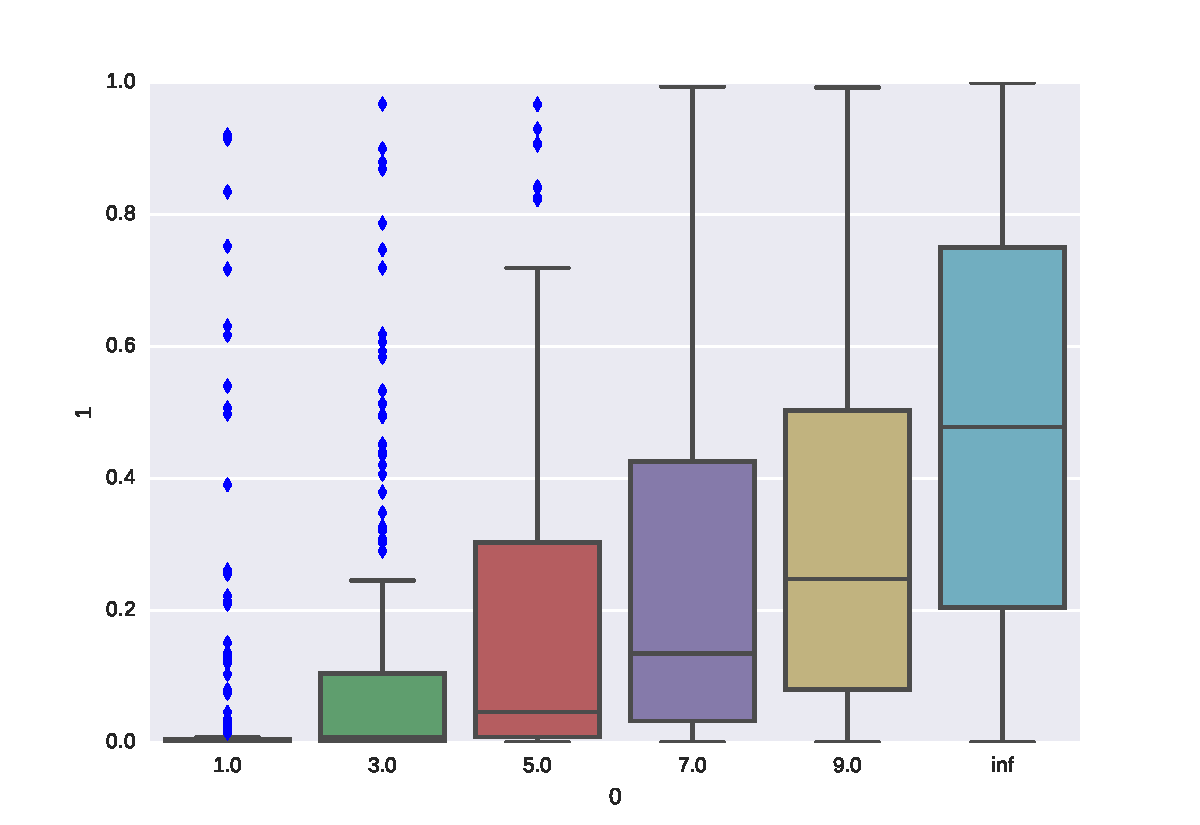
\includegraphics[width=0.8\textwidth]{img/student}
\caption{Linear Time test. Distribution of p-values as a function of number
of degrees of freedom.}
\end{figure}



\subsection{MCMC diagnostic}

This one sample test can be used for diagnostics of most of the MCMC
methods. In the following experiment we will demonstrate how to verify
if the samples obtained form two sampling can be assumed to come from
the stationary distribution.

Here we model used in the experiment 5.1. The model is 
\begin{align}
\theta_{1}\sim N(0,10);\theta_{2}\sim N(0,1)X_{i}\sim\frac{1}{2}N(\theta_{1},4)+\frac{1}{2}N(\theta_{2},4)
\end{align}
400 points are drawn from this model. In the following experiment
we would like to characterize the average time required for convergence
for two different MCMC algorithms. In order to do so we run multiple
chains and asses distribution of p-values. Under the null hypothesis
p-values should have uniform distribution and, as in the previous
experiment, we asses the divergence of the p-values from the uniform
by bar plots. Formally for both methods plain MH and SGLD we generate
$40\times100$ chains. We divide those chains into $40$ groups of
$100$ chains and run one-sample tests for for predefined times $t_{1},...,t_{1}0$
so that for each of group we get p-values at ten different times.
Then we plot those p-values jointly on plots a and b. We don't use
thinning.


\paragraph{Metropolis Hastings with random walk}

We use plain MH MCMC with Gaussian proposal with with standard deviation
equal to $0.2$.


\subsection{SGLD, plain }

Stochastic gradient Stochastic Gradient Langevin Dynamics with schrinking
step size $\epsilon_{t}$ is a MCMC procedure desigend for large datasets.
400 points are drawn from the this model with $\theta_{1}=0$ and
$\theta_{2}=1$. In such a setting there are two modes in the posteriori
disitbiution, one at the the point $0,1$ and the other at the point
$1,-1$. We run the SGLD alogrithm with a batch size of 1 and 10000
iterations through the whole dataset. The stepsizes are $\epsilon_{t}=a(b+t)^{.55}$
where $a=0.01584$ and $b=2.31$ such that $\epsilon_{t}$ deacreses
from $0.01$ to $.0001$.

\begin{figure}
\begin{centering}
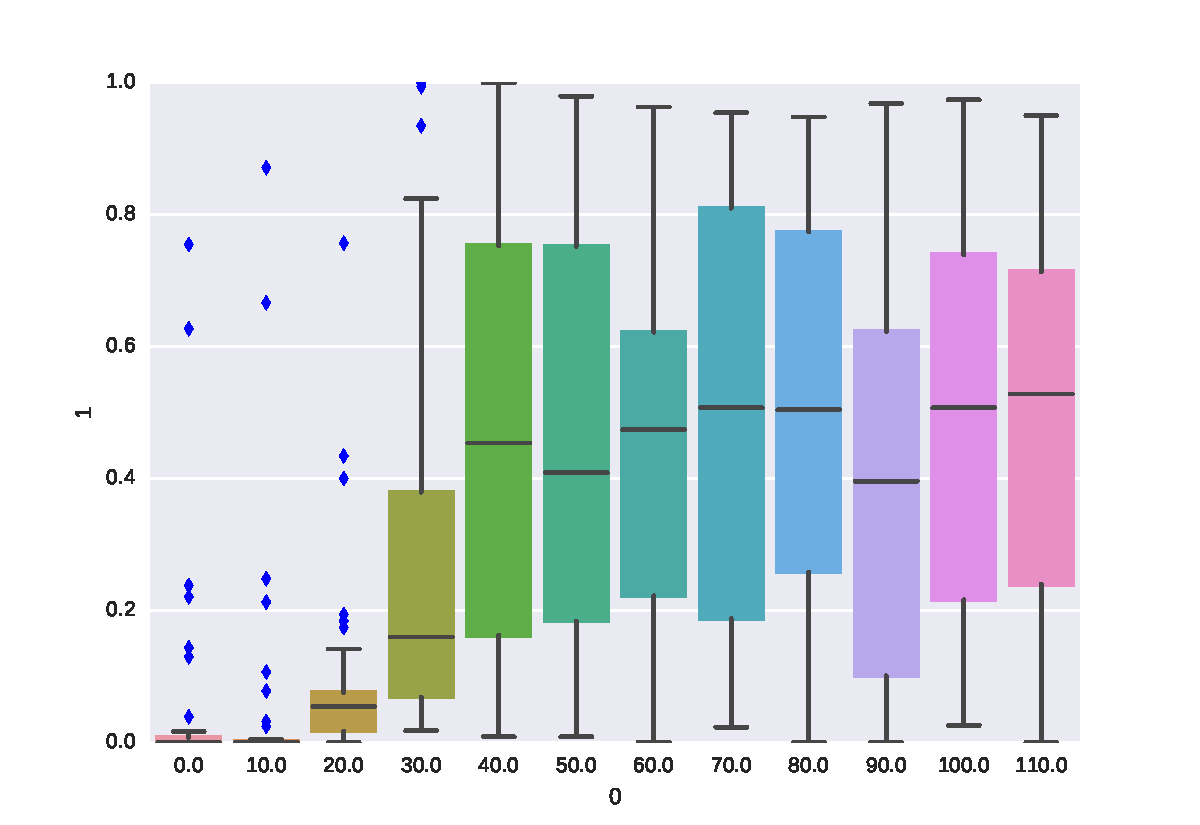
\includegraphics[width=7cm]{img/mcmc_mixing} 
\par\end{centering}

\centering{}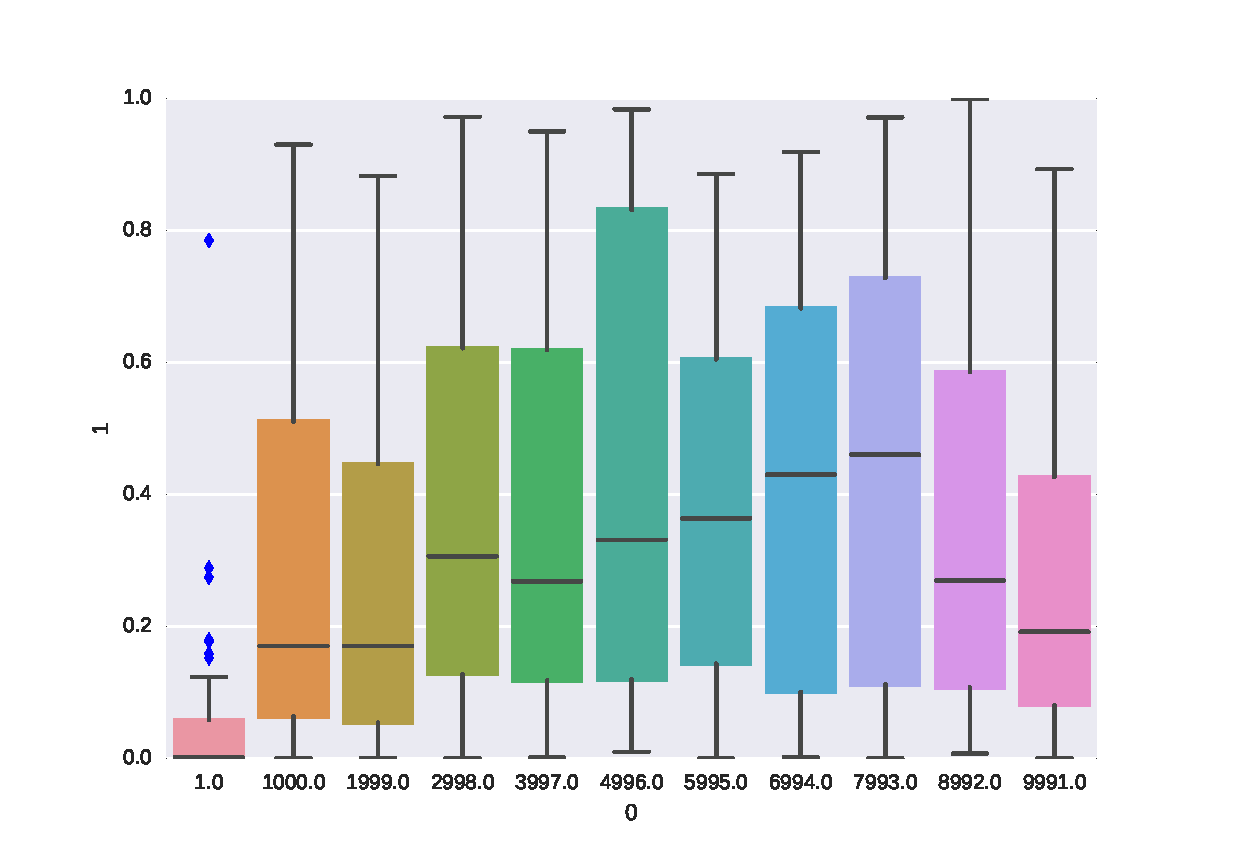
\includegraphics[width=7cm]{img/sgld_mixing} 
\end{figure}


\begin{figure}
\begin{centering}
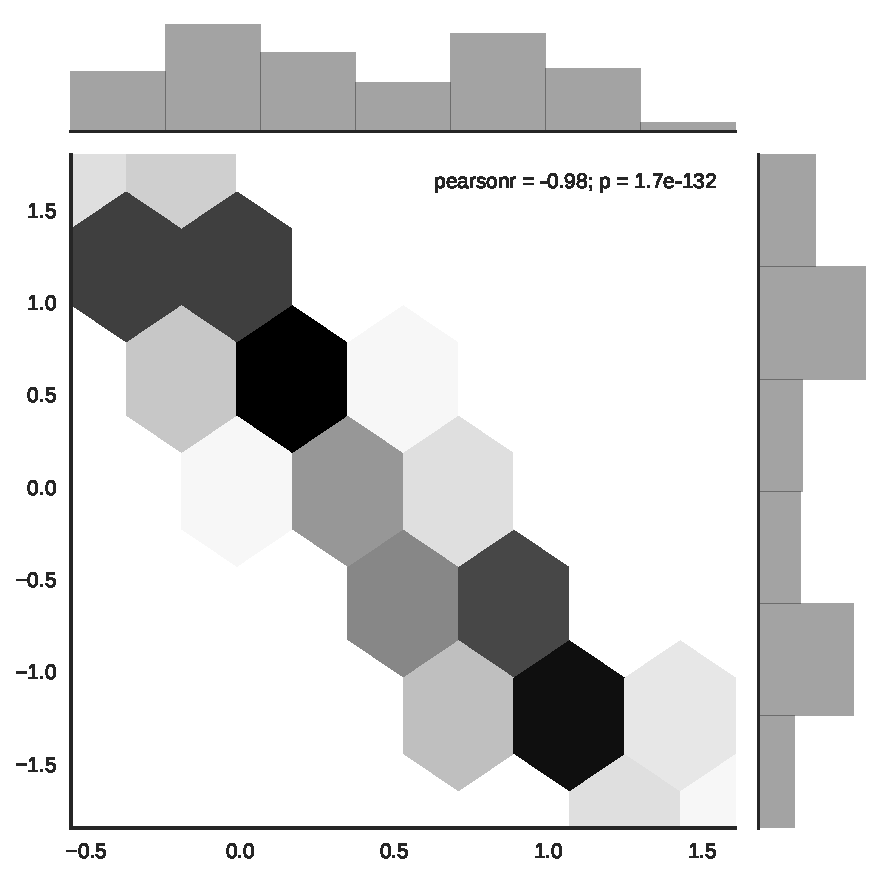
\includegraphics[width=7cm]{img/mcmc_sample}
\par\end{centering}

\centering{}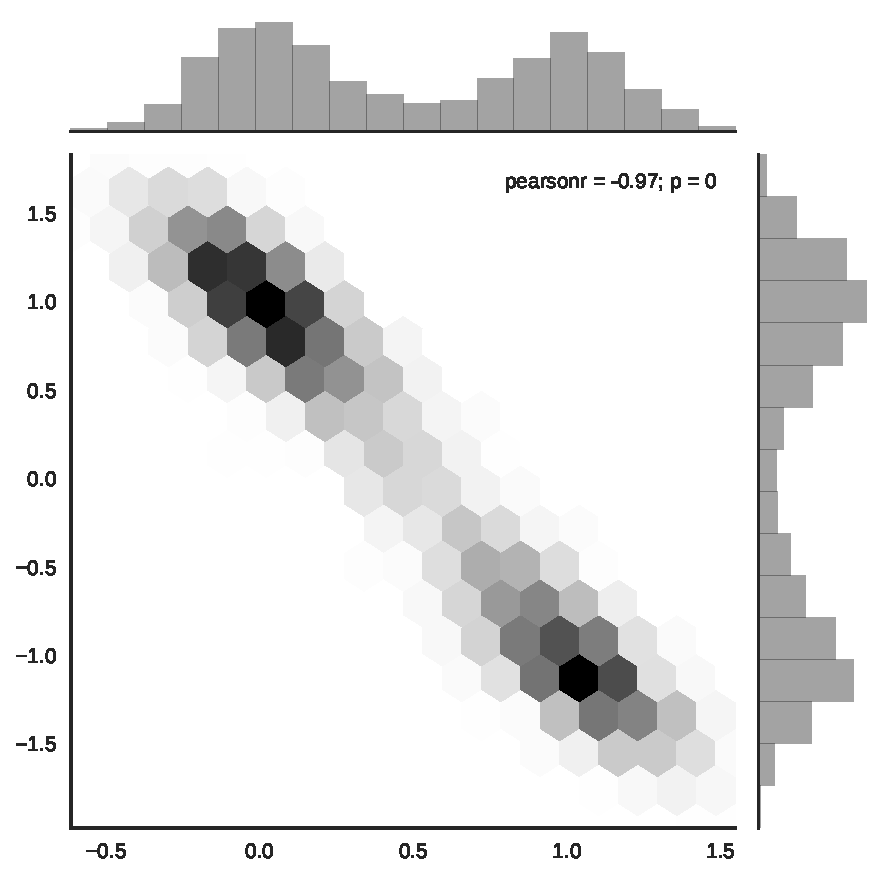
\includegraphics[width=7cm]{img/sgld_sample} 
\end{figure}


\selectlanguage{british}%

\section{Experiments}


\subsubsection*{Convergence in non-parametric density estimation}

Our next experiment illustrates using the developed test to asses
estimation quality in the context of nonparametricdensity estimation.
We quantify estimation quality and approximation quality of the infinite
dimensional exponential family model \citep{SriFukKumGreHyv14} and
its recent random Fourier features approximation \citep{strathmann2015gradient}
respectively.

The original model's (un-normalised) log pdf is given by $f(x)$ where
$f\in{\cal H}$ lies in a Reproducing Kernel Hilbert Space ${\cal H}$
induced by a Gaussian kernel with bandwidth 1. We fit the model to
$N$ standard Gaussian distributed data and perform our quadratic
time test on seperate test data of a fixed size $N_{\text{test}}=500$.
We aim to identify the number of samples necessary to make model and
data indistinguishable for a test of a certain power. Figure \ref{fig:density_estimation_increasing_data}
shows the distribution of p-values for this particualar test power
$N_{\text{test}}$ is uniform for $N=5000$, but already at $N=500$,
the null hypothesis would very rarely be rejected.

We now use the recent random Features approximation \citep{strathmann2015gradient}
where the log pdf is taken to be $\theta^{\top}\phi_{x}$ where $\theta\in\mathbb{R}^{m}$
and $\phi_{x}\in\mathbb{R}^{m}$ is the random Fourier feature embedding
\citep{Rahimi2007}. The natural question when using this approximation
is: ``How many random features do it I need?'' Using the same test
power $N_{\text{test}}=500$ as above, and a large number of available
samples $N=5\cdot10^{4}$, Figure \ref{fig:density_estimation_increasing_features}
shows the distribution of p-values for an increasing number of random
features $m$. From about $m=50$, the null hypothesis would rarely
be rejected for the chosen test power.

and \ref{fig:density_estimation_increasing_features} 
\begin{figure}
\begin{centering}
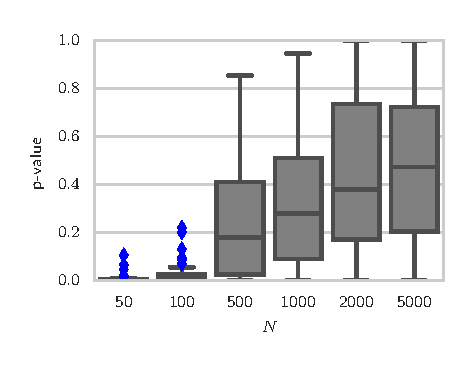
\includegraphics{img/increasing_data_fixed_test}
\par\end{centering}

\caption{P-values for an increasing number of data $N$ for the non-parametric
model.}


\label{fig:density_estimation_increasing_data}
\end{figure}
\begin{figure}
\begin{centering}
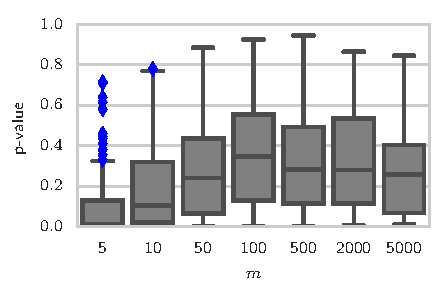
\includegraphics{img/increasing_features_fixed_test}
\par\end{centering}

\caption{P-values for an increasing number of random features $m$.}


\label{fig:density_estimation_increasing_features}
\end{figure}


\bibliographystyle{icml2015}
\bibliography{biblio}


\pagebreak{}

\normalsize\onecolumn


\part*{Appendix}

\selectlanguage{english}%

\section{boring proofs}
\begin{lem}
\label{lem:easy} If a random variable $X$ is distributed according
to $p$, then for all function $f\in\mathcal{F}$ expected value of
$T_{p}$ is zero, i.e. $\forall_{f\in\mathcal{F}}\ev(T_{q}f)(X)=0$.\end{lem}
\begin{proof}
First we show that the functions $g_{i}=p\cdot f_{i}$ vanish at infinity,
by which we mean that for all dimensions $j$ 
\[
\lim_{x_{j}\to\infty}g_{i}(x_{1},\cdots,x_{d})=0.
\]
The density function $p$ vanishes at infinity. The function $f$
is bounded, which is implied by Cauchy-Schwarz inequality -- $\left|f(x)\right|\le\left\Vert f\right\Vert \sqrt{k(x,x)}$.
This implies that the function $g$ vanishes at infinity. To show
the expected value $\ev(T_{p})f(X)$ is zero, it is sufficient to
show that for all dimensions $i$, the expected value of $\frac{\partial\log p(X)}{\partial x_{i}}f_{i}(X)+\frac{\partial f_{i}(X)}{\partial x_{i}}$
is zero. 
\begin{align*}
 & \ev\left(\frac{\partial\log p(x)}{\partial x_{i}}f_{i}(x)+\frac{\partial f_{i}(x)}{\partial x_{i}}\right)\\
 & =\int_{R_{d}}\left[\frac{\partial\log p(x)}{\partial x_{i}}f_{i}(x)+\frac{\partial f_{i}(x)}{\partial x_{i}}\right]q(x)dx\\
 & =\int_{R_{d}}\left[\frac{1}{p(x)}\frac{\partial q(x)}{\partial x_{i}}f(x)+\frac{\partial f(x)}{\partial x_{i}}\right]q(x)dx\\
 & =\int_{R_{d}}\left[\frac{\partial p(x)}{\partial x_{i}}f_{i}(x)+\frac{\partial f_{i}(x)}{\partial x_{i}}q(x)\right]dx\\
 & \overset{(a)}{=}\int_{R_{d-1}}\left(\lim_{R\to\infty}p(x)f_{i}(x)\bigg|_{x_{i}=-R}^{x_{i}=R}\right)dx_{1}\cdots dx_{i-1}\cdots dx_{i+1}\cdots d{x_{d}}\\
 & =\int_{R_{d-1}}0dx_{1}\cdots dx_{i-1}\cdots dx_{i+1}\cdots d{x_{d}}\\
 & =0.
\end{align*}
For the equation (a) we have used integration by parts and fact that
$g_{i}$ vanishes at infinity. 
\end{proof}

\subsection{Linear time}

For some fixed location $y$ and a random variable $X$, define a
random variable $s(X,y)$ 
\begin{align}
s(X,y)=\nabla\log p(X)g(X,y)-\nabla g(X,y).
\end{align}
For some number of random locations $Y_{1},Y_{J}$ and a random variable
$X$ define a random vector $Z_{i}$ 
\begin{equation}
Z_{i}=(s(X_{i},Y_{1}),\cdots,s(X_{i},Y_{J}))\in\mathbf{R}^{J}.
\end{equation}


Let $W_{n}$ be a mean of $Z_{i}$'s $W_{n}=\frac{1}{n}\sum_{i=1}^{n}Z_{i},$
and $\Sigma_{n}$ its covariance matrix $\Sigma_{n}=\frac{1}{n}ZZ^{T}$.
The test statistic is 
\begin{equation}
S_{n}=nW_{n}\Sigma_{n}^{-1}W_{n}.
\end{equation}
The computation of $S_{n}$ requires inversion of a $J\times J$ matrix
$\Sigma_{n}$, but this is fast and numerically stable: $J$ will
typically be small, and is less than 10 in our experiments. The next
proposition demonstrates the use of $S_{n}$ as a one-sample test.
\begin{prop}[\selectlanguage{english}%
Asymptotic behavior of $S_{n}$\selectlanguage{british}%
]
 \label{prop:Hotelling} If $\ev s(X,y)=0$ for all $y$, then the
statistic $S_{n}$ is a.s. asymptotically distributed as a $\chi^{2}$-random
variable with $Jd$ degrees of freedom, where $d$ is $X$ dimensionality
(as $n\to\infty$ with $d$ fixed). If $\ev s(X,y)\neq0$ for almost
all $y$ then a.s. for any fixed $r$, $\mathbb{P}(S_{n}>r)\to1$
as $n\to\infty$ . 
\end{prop}

\paragraph{One sample test}

Calculate $S_{n}$. Choose a threshold $r_{\alpha}$ corresponding
to the $1-\alpha$ quantile of a $\chi^{2}$ distribution with $J$
degrees of freedom, and reject the null hypothesis whenever $S_{n}$
is larger than $r_{\alpha}$. \selectlanguage{british}%

\end{document}
